\documentclass[12pt,a4paper]{article}
\usepackage[utf8]{inputenc} %polskie znaki
\usepackage[T1]{fontenc}	%polskie znaki
\usepackage{amsmath}		%matematyczne znaczki :3
\usepackage{enumerate}		%Dodatkowe opcje do funkcji enumerate
\usepackage{geometry} 		%Ustawianie marginesow
\usepackage{graphicx}		%Grafika
\usepackage{wrapfig}		%Grafika obok textu
\usepackage{float}			%Allows H in fugire
%\pagestyle{empty} 			%usuwa nr strony

\newgeometry{tmargin=2cm, bmargin=2cm, lmargin=2cm, rmargin=2cm} 

\begin{document}
	\begin{center}
		\LARGE Trygonometria
	\end{center}
	\vspace{1cm}
	
	
	\begin{enumerate}[1.]
		\item Wyznacz funkcje trygonometryczne kątów ostrych trójkąta egipskiego.
		
		\item Wyznacz funkcje trygonometryczne podanych kątów:
		
		\begin{figure}[h]
			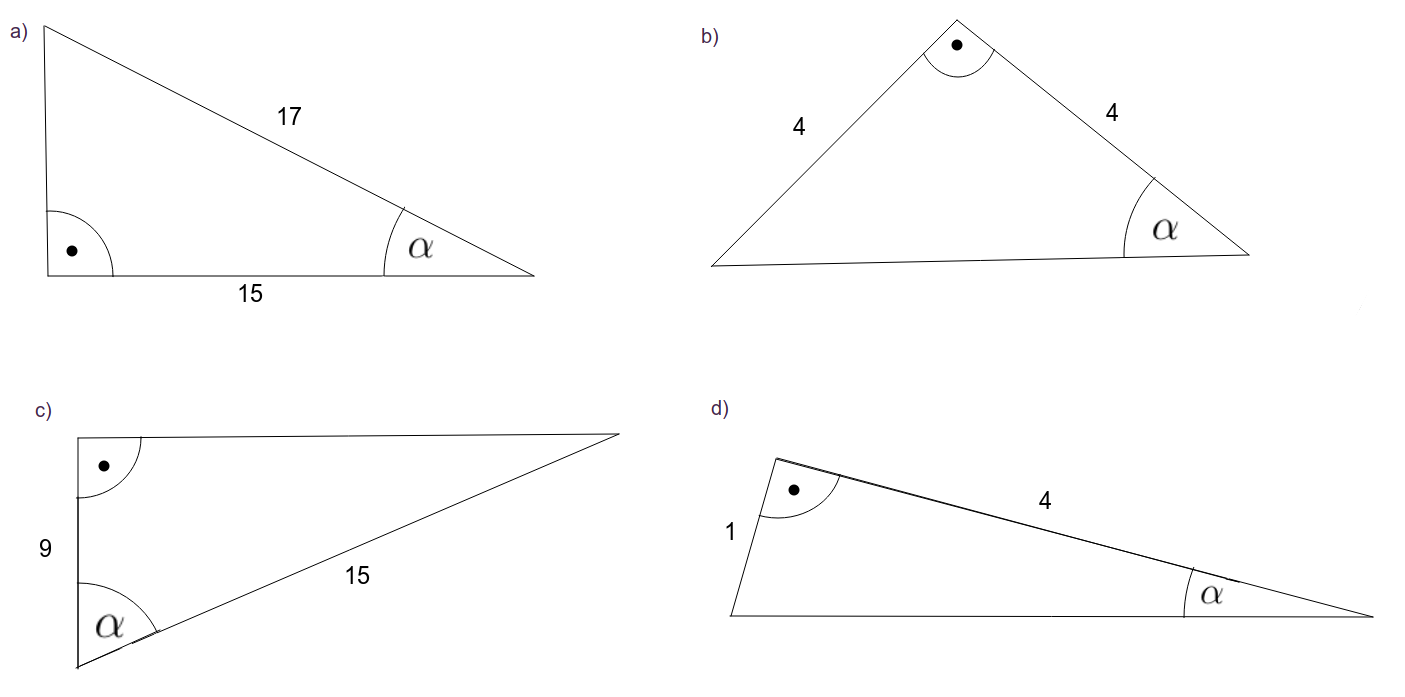
\includegraphics[scale=0.35]{t1}
		\end{figure}
	
		\item Oblicz brakujące boki:
		
		\begin{figure}[h]
			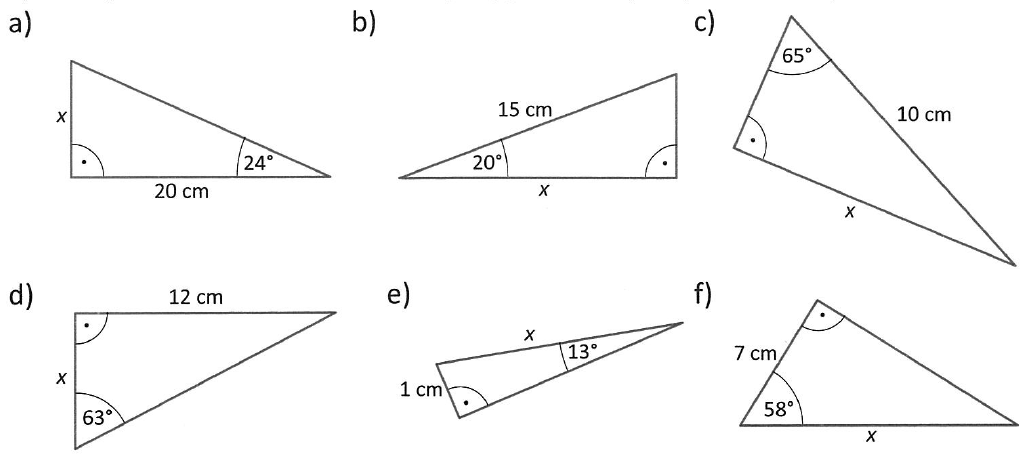
\includegraphics[scale=0.65]{t2}
		\end{figure}
	
			\item Dla podanej funkcji trygonometrycznej wyznacz jej pozostałe funkcje trygonometryczne:
	
		\begin{enumerate}[a)] \begin{tabular}{p{7cm} p{7cm}}
			\item $\sin\alpha=\frac{5}{13}$& \vspace{0.4cm} \item $\cos\alpha=0,5$ \\
			\item $\cos\alpha=\frac{\sqrt{5}}{5}$& \item $\text{ctg } \alpha=\frac{1}{\sqrt{3}}$ \\
			\item $\text{tg }\alpha=2$& \item $\sin\alpha=\frac{1}{\sqrt{3}}$ \\
		\end{tabular} \end{enumerate}
	
		\item W równoległoboku $ABCD$ wysokości mają długości 4 cm i 5 cm, a kąt rozwarty ma $115^\circ$. Oblicz obwód tego równoległoboku.
		
		\item Pewne promienie słoneczne padają na drzewo pod kątem $25^\circ$. Wiedząc, że drzewo rzuca cień od długości 30m, oblicz wysokość tego drzewa.
		
		\item Pewne promienie słoneczne padają pod kątem $16^\circ$ na masz o wysokości 15,5m. Oblicz długość cienia który rzuca maszt.
		
		\item Oblicz:
		
		\begin{enumerate}[a)]
			\item $4\cdot \cos(60^\circ)\cdot \sin(30^\circ)-\cos(30^\circ)\cdot\sin(30^\circ)=$
			\item $\text{ctg }(30^\circ)\cdot\text{ctg }(45^\circ):(\text{ctg }(60^\circ)\cdot \text{tg }(45^\circ))=$
			\item $18\cdot \sin(30^\circ)\cdot\text{tg }(30^\circ):(\cos(30^\circ)\cdot\text{tg }(60^\circ))=$
			\item $6\cdot (\sin(30^\circ)\cdot\cos(45^\circ)\cdot\text{ctg }(60^\circ)):(\text{ctg }(30^\circ)\cdot\sin(45^\circ))=$	
			\item $12\cdot(\text{tg }(60^\circ)-\cos(60^\circ))\cdot(\text{tg }(30^\circ)+\text{tg }(30^\circ)+\cos(30^\circ))=$	
			\item $(\sin(45^\circ)+\text{ctg }(45^\circ))\cdot(6\cdot\sin(60^\circ)-\text{ctg }(30^\circ))=$	
			\item $(\cos(45^\circ)-\cos(30^\circ))\cdot(\cos(45^\circ)+\cos(30^\circ))=$
			\item $(3\cdot \sin(45^\circ)+\text{tg }(60^\circ))\cdot(3\sin(45^\circ)-\text{tg }(60^\circ))=$
			\item $(\sin(60^\circ)+\cos(30^\circ))^2-(\sin(30^\circ)+\cos(60^\circ))^2=$
		\end{enumerate}
	
		\item Sprawdź, czy podana równość jest tożsamością trygonometryczną:
		
		\begin{enumerate}[a)]
			\item $\text{tg }\alpha\cdot\cos\alpha=\sin\alpha$
			\item $\sin\alpha(\frac{1}{\sin\alpha}-\sin\alpha)=\cos^2\alpha$
			\item $1-2\sin^2\alpha=2\cos^2\alpha$
			\item $\sin\alpha+\sin\alpha\cdot\text{tg }^2\alpha=\frac{\text{tg }\alpha}{\cos\alpha}$
		\end{enumerate}

	\end{enumerate}
\end{document}